\documentclass[10pt,a4paper,hidelinks]{article}
\usepackage{lipsum}
\usepackage[bahasai,bahasa]{babel}
\selectlanguage{bahasai}
\usepackage{url}
\usepackage{graphicx}
\usepackage[nochapters]{classicthesis} % nochapters
\usepackage{babelbib}
\selectbiblanguage{bahasa}
\setbtxfallbacklanguage{bahasa}
\usepackage{mhchem}
\usepackage{standalone}
\usepackage{flowchart}
\usepackage{tikz}
\usepackage{pgfgantt}
\usetikzlibrary{arrows,calc,positioning}

%TikZ
\tikzstyle{intt}=[draw,text cenStered,minimum size=6em,text width=5.25cm,text height=0.34cm]
\tikzstyle{intl}=[draw,text centered,minimum size=2em,text width=2.75cm,text height=0.34cm]
\tikzstyle{int}=[draw,minimum size=2.5em,text centered,text width=3.5cm]
\tikzstyle{intg}=[draw,minimum size=3em,text centered,text width=6.cm]
\tikzstyle{sum}=[draw,shape=circle,inner sep=2pt,text centered,node distance=3.5cm]
\tikzstyle{summ}=[drawshape=circle,inner sep=4pt,text centered,node distance=3.cm]

\begin{document}
    \pagestyle{plain}
    \title{\rmfamily\normalfont\spacedallcaps{Meningkatkan Efisiensi Pengolahan Limbah Air melalui proses hibrida dengan Microbial Fuel Cell}}
    \author{\spacedlowsmallcaps{Eko J. Salim \& Gerraldo S. Candra}}
    \date{} % no date
    
    \maketitle
    
    \begin{abstract}
    	\noindent Proses pengolahan limbah air sekarang meninggalkan banyak ruang untuk dikembangkan dan ditingkatkan. Limbah dapat menjadi sumber energi yang berharga --- sekitar 9 kali lebih banyak energi terkandung dalam limbah dibandingkan dengan energi yang diperlukan untuk mengolahnya dengan cara modern. Proses-proses yang tersedia sekerang jarang mempertimbangkan dan menggunakan hal ini, proses-proses ini juga sering tidak efisien dan 'kotor'.
Menggabungkan teknologi-teknologi pengolahan limbah menjadi sebuah proses hibrida berpusat pada Microbial Fuel Cell (MFC) dapat memecahkan masalah ini. Keuntungan yang didapat dalam menggunakan proses hibrida ini diantara lain adalah berikut: ekstraksi sumber daya, ekstraksi energi (listrik) yang lebih besar dan efisien dan pembersihan limbah yang lebih bersih.
       % \noindent Current wastewater treatment processes and technologies left much to be desired. Wastewater could be a valuable source of energy --- about 9 times more energy are in wastewater compared to the energy needed to proccess them in a modern plant. Present processes do not generally take this into account moreover, they are also generally inefficient and 'unclean'. Combining present technologies, such as and especially Microbial Fuel Cell (MFC) could help alleviate these present issues considering wastewater treatment. 
    \end{abstract}
       
    \tableofcontents
    \section{Pendahuluan}
    \subsection{Latar Belakang}
    Proses pengolahan limbah air yang ada sekarang tidak dapat memenuhi aspirasi masyarakat yang menginginkan air bersih, energi dan sumber daya dari limbah. Proses sekerang malah menggunakan energi yang signifikan. Konsumsi energi dari industri air diperkirakan adalah 2\% dari konsumsi listrik global. Penting sekali adanya proses pengolahan yang lebih efisien dalam konteks energi. Menurut Perserikatan Bangsa-Bangsa, diperkirakan tindakan mengingkatkan efisiensi adalah 65\% dari penghematan emisi global sampai dengan 2030.
    
    Dalam proses-proses yang menghemat energi ini, juga diharapkan kalau dapat diperoleh energi dan sumber daya dari limbah. Mengingat pentingnya mendaur ulang energi dan sumber daya untuk kelangsungan peradaban manusia sekarang ini, pendauran ulang dari limbah sangat diharapkan.
    
	\subsection{Identifikasi Masalah}
	\begin{itemize}
	\item Proses pengolahan limbah air sekarang tidak dapat memenuhkan aspirasi masyarakat
	\item Dari proses pengolahan limbah air, diharapkan didapatkannya energi, air bersih dan sumber daya
	\item Proses yang ada sekarang tidak hemat energi, 2\% dari total konsumsi listrik global adalah untuk air
	\item Penting didaur-ulangnya sumber daya dan energi dari limbah untuk memecahkan masalah energi dunia
	\end{itemize}
	\subsection{Batasan Masalah}
	Memperoleh air bersih, energi dan sumber daya dari limbah air
	\subsection{Rumusan Masalah}
	Bagaimana sebuah proses hibrida yang dapat mengolah limbah air dengan optimal?
	\subsection{Tujuan Penelitian}
	\subsubsection{Tujuan Umum}
	Diperolehnya proses / rangkain proses yang sesuai dan optimal untuk digunakan dengan Microbial Fuel Cell untuk memaksimalkan sepenuhnya ekstraksi (air bersih, energi, sumber daya, dan lain lain) dari limbah dengan efisien.
	\subsubsection{Tujuan Khusus}
	\begin{itemize}
	\item Mengidentifikasi masalah yang muncul dari proses hibrida dan solusi yang memungkinkan
	\item Mencari solusi rangkain proses yang seekonomis mungkin untuk digunakan di masyarakat
	\item Mengidentifikasi kelemahan dan kelebihan dari proses-proses dan teknologi pengolahan limbah
	\item Meneliti kesesuaian Microbial Fuel Cell dengan proses-proses pengolahan limbah lainnya
	\item Memperoleh data penggunaan sistem Microbial Fuel Cell dengan berbagai tipe limbah
	\end{itemize}
	\subsection{Manfaat Penilitian}
	Dengan penelitian ini, diharapkan rangkaian proses yang sesuai dan efektif dapat ditemukan dan dievaluasi sehingga dapat digunakan oleh masyarakat dan juga diteliti lebih lanjut.
	\section{Tinjauan Pustaka}
    \subsection{Kajian Teori}
    Banyak teknologi dapat digunakan untuk pengolahan limbah: dari sistem  \textit{activated sludge} sampai \textit{vacuum evaporation}. Menggabungkan teknologi-teknologi yang ada ini menjadi sebuah sistem hibrida dengan Microbial Fuel Cell dapat menghasilkan sebuah proses pengolahan limbah yang berkelanjutan.
    %Various technologies are available for wastewater treatment: from activated sludges to vacuum evaporation. Combining these technologies below could lead into a sustainable wastewater treatment especially in a MFC-centered treatment process.
    \subsubsection{Microbial Fuel Cell}
    Microbial Fuel Cell adalah alat yang menghasilkan arus menggunakan bakteri. bakteri di dalam MFC bekerja sebagai sebuah katalis untuk mengoksidasi zat organik maupun zat anorganik. Elektron hasil dari oksidasi ini bergerak menuju elektroda dan akhirnya menuju katoda dari anoda. Bagaimana cara elektron ditransfer ke anoda adalah perbedaan antara MFC dengan penengah dan tanpa penengah. Di MFC dengan penengah, ada penengah redox yang mengangkut elektron ke anoda. Jika tidak ditambah mediator eksogen, MFC tersebut dikatakan sebagai MFC tanpa penengah. Dalam MFC tanpa penegah, transfer elektron bisa dilakukan dengan cara: \textit{direct membrane associated electron transfer}, \textit{bacteria's nanowire}, dll. 
    %Microbial fuel cells are devices that drives a current using bacterias. Bacterias in a microbial fuel cell serve as catalyst to oxidize both organic and inorganic matters.  The electrons from this oxidation are transferred to the anode and then to the cathode.  The 'how' electrons are transferred to anode serves as the distinction between two general types of MFC. In mediator microbial fuel cell, there exists a redox mediator which ‘shuttles’ electrons to the anode. A microbial fuel cell is classified as a mediator-less MFC if no exogenous mediators are added,  the method ofelectrons transfer in these instances can be by the following: direct membrane associated electron transfer, bacteria’s ‘nanowires’ . . .


Di hampir semua MFC, elektron yang mencapai katoda bergabung dengan proton yang membaur dari anoda dna juga dengan oksigen dari udara; produk hasil penggabungan ini adalah air. Oksidator kimia juga dapat digunakan.
%In most MFCs, the electrons that reach the cathode combine with protonsthat diffuse from the anode and oxygen provided from the  air;  the  resulting  product  is  water.   Chemical  oxidizers  may  also  be used however because they need to replaced, they are not practical outisde laboratory use.


Karena MFC 'memakan' zat organik dan anorganik dan juga memproduksi listrik, MFC dapat digunakan dalam pengolahan limbah. Banyak riset telah meneliti tentang MFC dan pengolahan limbah, dari efektivitasnya dalam mengolah limbah intensitas tinggi sampai menambahkan efektivitas MFC dengan \textit{spiral spacer}.
%As MFCs break down organic matters and produce electricity, MFCs have found a use in wastewater treatment.


Dalam proses pengolahan berbasis MFC, kelemahan dan kelebihan MFC  harus dipertimbangkan. MFC yang sekarang kurang cocok dalam mengolah limbah intensitas tinggi. Isu \textit{scaling} juga adalah sebuah kelemahan MFC. Dengan menggabungkan teknologi MFC dengan teknologi lain, kita dapat mengatasi kelemahan-kelemahan dari MFC.
%In MFC-centered treatment process, weaknesses and advantages of MFC must be considered. MFC technologies fall short in treating high-intensity wastewater/sludge and scaling. However, numerous researches have proposed many and various solutions to MFC's shortcoming. 
	\begin{figure}[!ht]
	\centering
		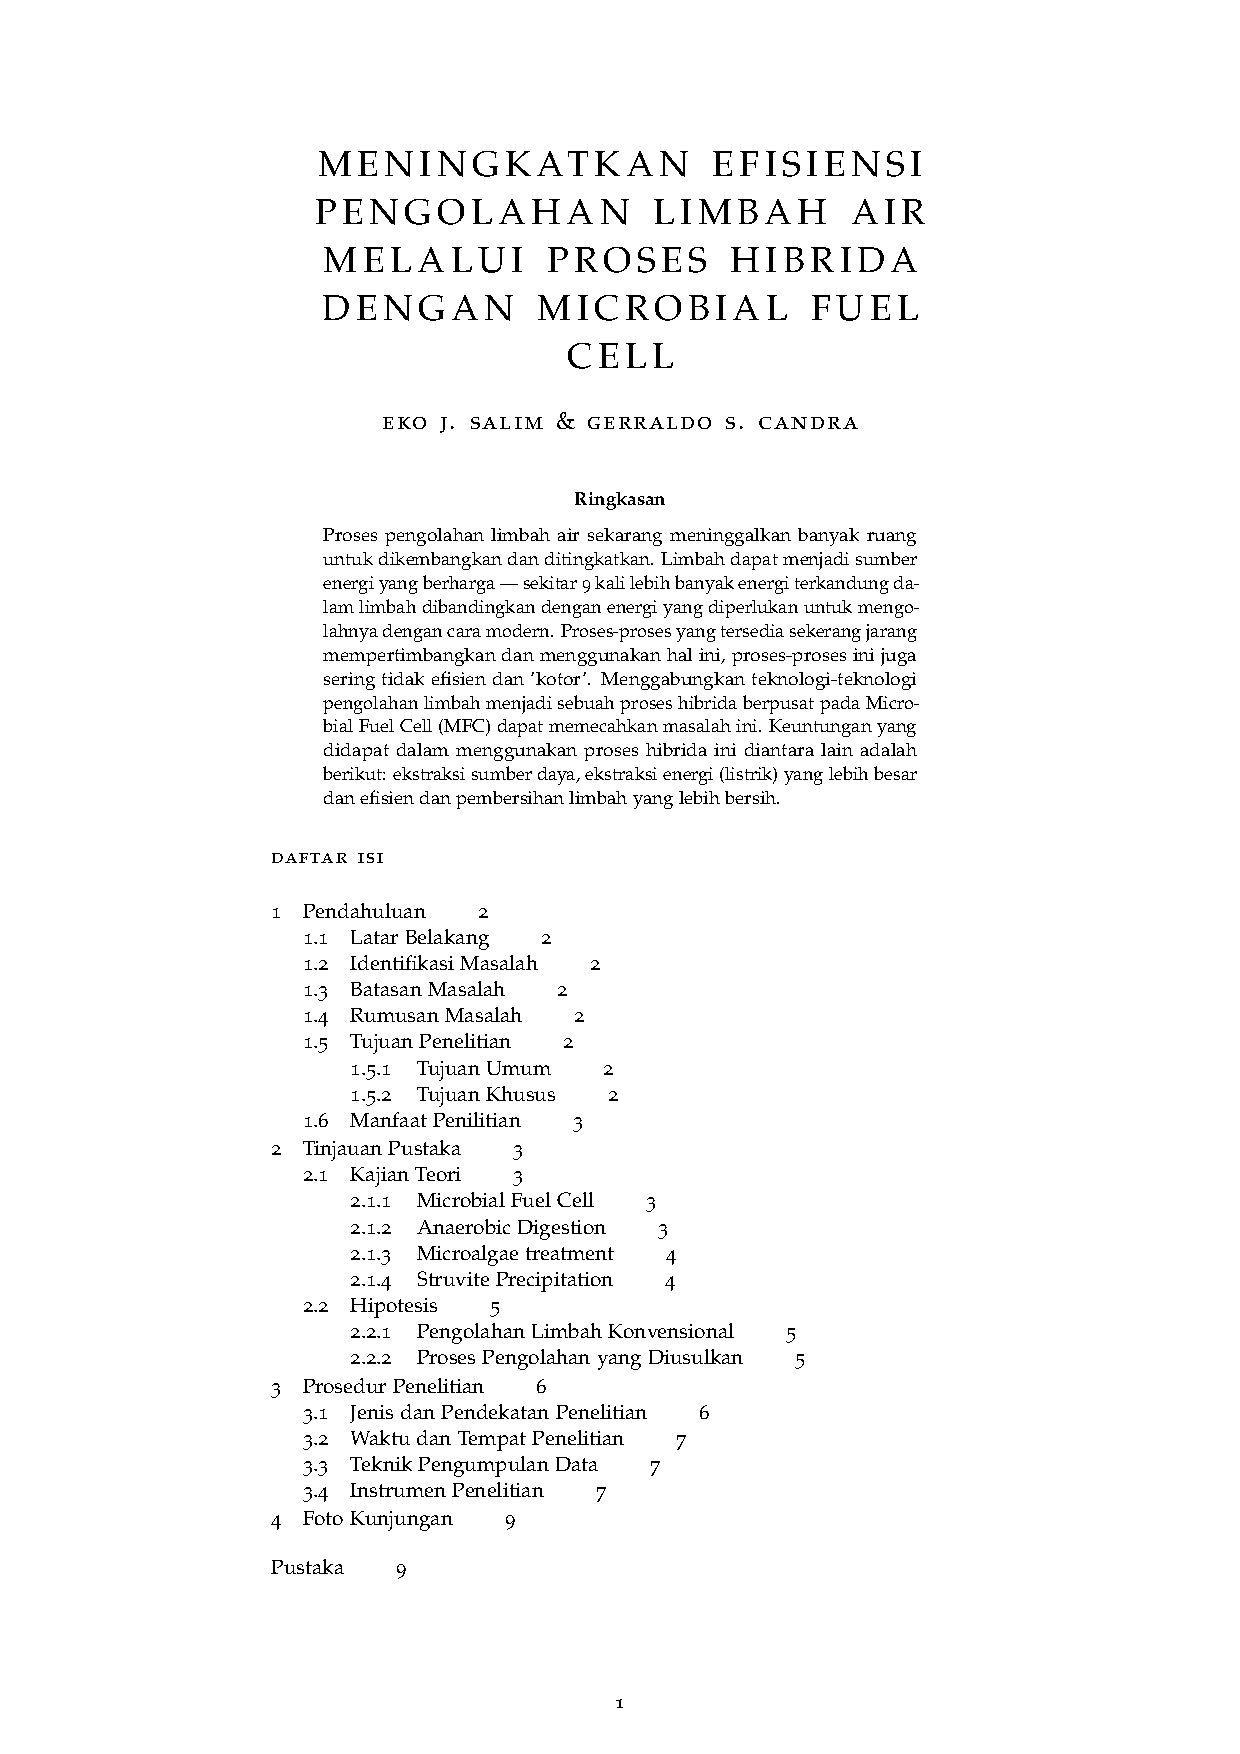
\includegraphics[scale=0.75]{gfx/mfc}
		%\caption{A bacterium in  the  anode  compartment  transfers electrons  obtained  from  an electron donor(glucose) to the anode electrode. This occurs either through direct contact, nanowires, or mobile electron shuttles (small spheres represent the final membrane associated shuttle). During electron  production  protons are  also  produced  in  excess.  These protons migrate through the cation exchange membrane (CEM) into the cathode chamber. The electrons flow from the anode through an external resistance (or load) to the cathode where they react with the final electron acceptor (oxygen) and protons}
		\caption{Sebuah bakteri dalam anoda mentransfer elektron yang didapat dari sebuah donor elektron menuju ke elektroda anoda. Dalam produksi elektron, proton juga diproduksi. Proton ini bergerak melalui sebuah membran pertukaran kation (\textit{cation exchange membrane}) menuju ke katoda. Elektron bergerak menuju katoda dimana kemudian mereka bereaksi dengan penerima elektron (oksigen) dan proton}
	\end{figure}
    \subsubsection{Anaerobic Digestion}
    Anaerobic digestion atau pencernaan anaerobik adalah proses dimana bakteri memecah zat \textit{biodegradable} saat tidak adanya oksigen. Pencernaan anaerobik dapat menghasilkan metana. Proses ini dimulai dengan hidrolisis oleh bakteri, polimer organik bersifat tidak larut diolah untuk digunakan bakteri lain. Bakteri \textit{acidogenic} mengubah gula dan asam amino menjadi asam asetat dan juga ammonia, hidrogen dan karbon dioksida. Kemudian, produk ini diubah menjadi metana dan karbon dioksida. Metana yang dihasilkan ini dapat digunakan untuk menghasilkan listrik.
    
Pecernaan anaerobik sudah dibuktikan dapat mengolah limbah intensitas tinggi, salah satu kelemahan dari MFC. Dari pengolahan limbah intensitas tinggi, hasilnya dapat digunakan oleh MFC untuk menghasilkan listrik dan lebih membersihkannya.
    \subsubsection{Microalgae treatment}
    Microalgae atau mikroalga dapat menjadi proses olahan setelah proses MFC. Mikroalga dapat mengolah nutrisi dan logam berat serta juga kontaminan dan polutan lainnya. Hasil olahan dari proses mikrolaga adalah biomassa yang dapat digunakan untuk produksi listrik. Mikrolaga juga menjadi sebuah opsi yang menarik karena kemampuannya untuk berkembang dengan nitrogen dan fosfor yang mereka olah.
    
	\begin{figure}[!ht]
	  \centering
		  \includegraphics[width=0.75\textwidth]{gfx/microalgae}
	  \caption{Mikroalga}
	\end{figure}

    \subsubsection{Struvite Precipitation}
    Nitrogen dan Fosfat harus disingkirkan atau diambil kembali sebuah mungkin dalam sebuah proses pengolahan limbah untuk memenuhi syarat-syarat, yang syarat utamanya adalah mencegah kerusakan lingkungan oleh eutrofikasi. \textit{Struvite Precipitation} adalah satu cara untuk memenuhi syarat ini. Struvite atau \ce{NH4MgPO4.6H2O} dapat diekstrak dari air limbah untuk memnuhi syarat penyingkiran nitrogen dan fosfor. Struvite juga dapat digunakan sebagai pupuk.
    \subsection{Hipotesis}
    \subsubsection{Pengolahan Limbah Konvensional}
    Dalam sebuah sistem pengolahan limbah air, tujuan utamanya adalah untuk menghilangkan BOD (\textit{Biochemical Oxygen Demand}), padatan tersuspensi, nutrisi-nutrisi, bakteri koliform dan zat berbahaya. Tujuan ini adalah untuk mendapatkan hasil yang bersih. Berikut ini adalah diagram proses pengolahan konvensional.
    
    \begin{center}
    \begin{tikzpicture}[>=latex',font={\sf \small}]
    \def\smbwd{4cm}
    \node (process1) at (0,0) [draw, process,minimum width=\smbwd, minimum height=1cm] {Pengolahan Awal};
    \node (process2) at (0,-2) [draw, process,minimum width=\smbwd, minimum height=1cm] {Pengolahan Primer};
    \node (process3) at (0,-4) [draw, process,minimum width=\smbwd, minimum height=1cm] {Pengolahan Sekunder};
    \node (process4) at (0,-6) [draw, process,minimum width=\smbwd, minimum height=1cm] {Pengolahan Tersier};
    \draw[->] (process1) -- (process2);
    \draw[->] (process2) -- (process3); 
    \draw[->] (process3) -- (process4);    
    \end{tikzpicture}
    \end{center}
    Pengolahan awal adalah untuk menyingkirkan benda padat besar yang ada pada air limbah.
    
    Pada pengolahan primer, air limbah akan melewati tanki/bak sedementasi. Tujuan dari bak sedementasi adalah untuk mengendap zat padat yang dapat mengendap. Dalam pengendapan ini, sampai dengan 40\% dari BOD dapat disingkirkan.
     
    Pengolahan sekunder bertujuan untuk mengurangi BOD dengan mengurangi zat organik.
    
    Pengolahan tersier bertujuan untuk menyingkirkan semua ion organik.
    
    Selain keempat proses ini, terdapat lagi pengolahan kuaterner dan juga disinfeksi. Pengolahan kuaterner bertujuan untuk menyingkirkan logam berat dan senyawa organik. Disinfeksi adalah penyingkiran semuah patogen. Disinfeksi biasa dilakukan dengan klorin/sinar UV.
    \subsubsection{Proses Pengolahan yang Diusulkan}
    Proses pengolahan yang ada kurang efisien dalam pengolahannya. Adanya kebutuhan energi yang tinggi yang sebagian besar karena kebutuhan aerasi. Ekstraksi sumber daya yang berguna juga masih minimal. Rangkaian proses dibawah ini seharusnya dapat membuat pengolahan air limbah menjadi lebih efisien.
    \begin{center}
    \begin{tikzpicture}[>=latex',auto]
    \node [intg] (kp1)  {Pengolahan Awal};
    \node [intg] (kp) [node distance=2cm and -1cm, below of=kp1]  {Pengolahan Primer};
      \node [int]  (ki2) [node distance=1.5cm and -1cm,below right=of kp] {UASB\\(Anaerobic Digestion)};
      \node [int]  (ki1) [node distance=2cm and -1cm,below of= ki2] {Struvite Precipitation};
      \node [intg] (ki3) [node distance=7cm,below of=kp] {Microbial Fuel Cell};
      \node [intg] (ki4) [node distance=2cm,below of=ki3] {Microalgae Treatment};
      \node [intg] (ki5) [node distance=2cm,below of=ki4] {Disinfeksi};

      \draw[->] (kp) -- ($(kp.south)+(0,-3)$) -| (ki3) node[left,pos=0.25] {Intensitas rendah-sedang} ;
      \draw[->] (kp) -- ($(kp.south)+(0,-0.75)$) -| (ki2) node[above,pos=0.35] {Intensitas tinggi \& Kaya Nutrisi};
      \draw[->] (kp1) -- (kp);
      \draw[->] (ki2) -- (ki1);
      \draw[->] (ki1) |- (ki3);
      \draw[->] (ki3) -- (ki4);
      \draw[->] (ki4) -- (ki5);
    \end{tikzpicture}
    \end{center}
    Microbial fuel cell menjadi pusat dari proses ini. Tenaga listrik dapat dihasilkan oleh Microbial Fuel Cell dan juga metana dari Anaerobic Digestion. Air limbah intensitas tinggi akan diproses oleh UASB karena teknologi MFC yang kurang cukup untuk menangani air limbah intensitas tinggi.
    
    
    Dari UASB (\textit{Upflow Anaerobic Sludge}) akan dilakukan \textit{Struvite Precipitation} untuk mengambil struvite yang akhirnya akan menjadi pupuk.
    
    
    Microbial Fuel Cell akan menghasilkan listrik dan pembersihan air limbah dari zat organik. MFC sekarang masih memiliki banyak kelemahan, \textit{Microalgae treatment} akan melakukan sentuhan terakhir untuk proses-proses sebelumnya. Mikroalga akan melakukan penyingkiran nutrisi nitrogen dan fosfor, pengurangan terakhir BOD, penyingkiran bakteri koliform, dan penyingkiran logam berat. \textit{Activated Sluge} dapat menjadi alternatif bagi tahap mikroalga tetapi, mikroalga lebih hemat energi karena tidak memerlukan aerasi.
    
    
    Setelah proses mikroalga, dapat dilakukan disinfeksi untuk memnuhi syarat kebersihan. Disinfeksi disarankan menggunakan sinar UV atau proses \textit{ozonation} karena naiknya harga klorin dan bahayanya terhadap ikan. Filtrasi terakhir juga dapat dilakukan untuk meningkatkan kualitas air.
    \section{Prosedur Penelitian}
    \subsection{Jenis dan Pendekatan Penelitian}
    Pendekatan yang akan digunakan adalah pendekatan secara kuantitatif dan jenis penelitian adalah penelitian berbasis eksperimen.
    \subsection{Waktu dan Tempat Penelitian}
    Estimasi waktu penelitian adalah 6 bulan.\\

    \begin{tikzpicture}[x=.5cm, y=1cm]
    \begin{ganttchart}{1}{12}
\gantttitle{2016}{12} \\
\gantttitlelist{1,...,6}{2}\\
\ganttgroup{Lama Penelitian}{2}{11} \\
 %%%%%%%%%%%%%%%%%Phase-1
\ganttbar{Pembuatan proposal}{2}{2} \\
\ganttlinkedbar{Pengumpulan data \& Bimbingan}{4}{10} \\
\ganttlinkedbar{Pembuatan prototype}{4}{10} \\
\ganttlinkedbar{Penyusunan Laporan}{11}{11} \ganttnewline

%%%%%%%%%%%%%%%%%%%%%%%%%%%%%%%%%%%%%%%%%%%%%%%%%%%%%%%%%%%%%%%
\end{ganttchart}  
\end{tikzpicture} 
    \\Tempat penelitian mencangkup:
    \begin{itemize}
    \item Instalasi Pengolahan Air Kotor (IPAK) Rawa Buaya, Cengkareng
    \item Fasilitas pengolahan limbah RS Siloam, Kebon Jeruk
    \item Fasilitas pengolahn limbah RS Puri, Puri Kembangan
    \item \textit{Centralized Treatment Plant} Lippo Karawaci
 	\item SMP Narada
    \end{itemize}
    
    \subsection{Teknik Pengumpulan Data}
    Teknik yang akan digunakan adalah eksperimen. Data juga akan didapat dari berbagai sumber artikel penelitian. Data yang diambil diantara lain adalah:
    \begin{itemize}
    \item COD \& BOD hasil dari sebuah proses pengolahan dan proses keseluruhan
    \item (Jumlah) Energi hasil proses \textit{Microbial Fuel Cell}
    \item Jumlah \textit{Struvite}(\ce{NH4MgPO4.6H2O}) yang terproduksi
    \item Jumlah gas metana yang terproduksi
    \item Rangkaian proses pengolahan
    \end{itemize}
    \subsection{Instrumen Penelitian}
    \begin{itemize}
    \item Unit Microbial Fuel Cell
    \item Kultur Mikroalga
    \item Reaktor \textit{Anaerobic Digestion}
    \item Sampel air limbah
    \end{itemize}
    \section{Foto Kunjungan}
    \begin{figure}[!ht]
	  \centering
		  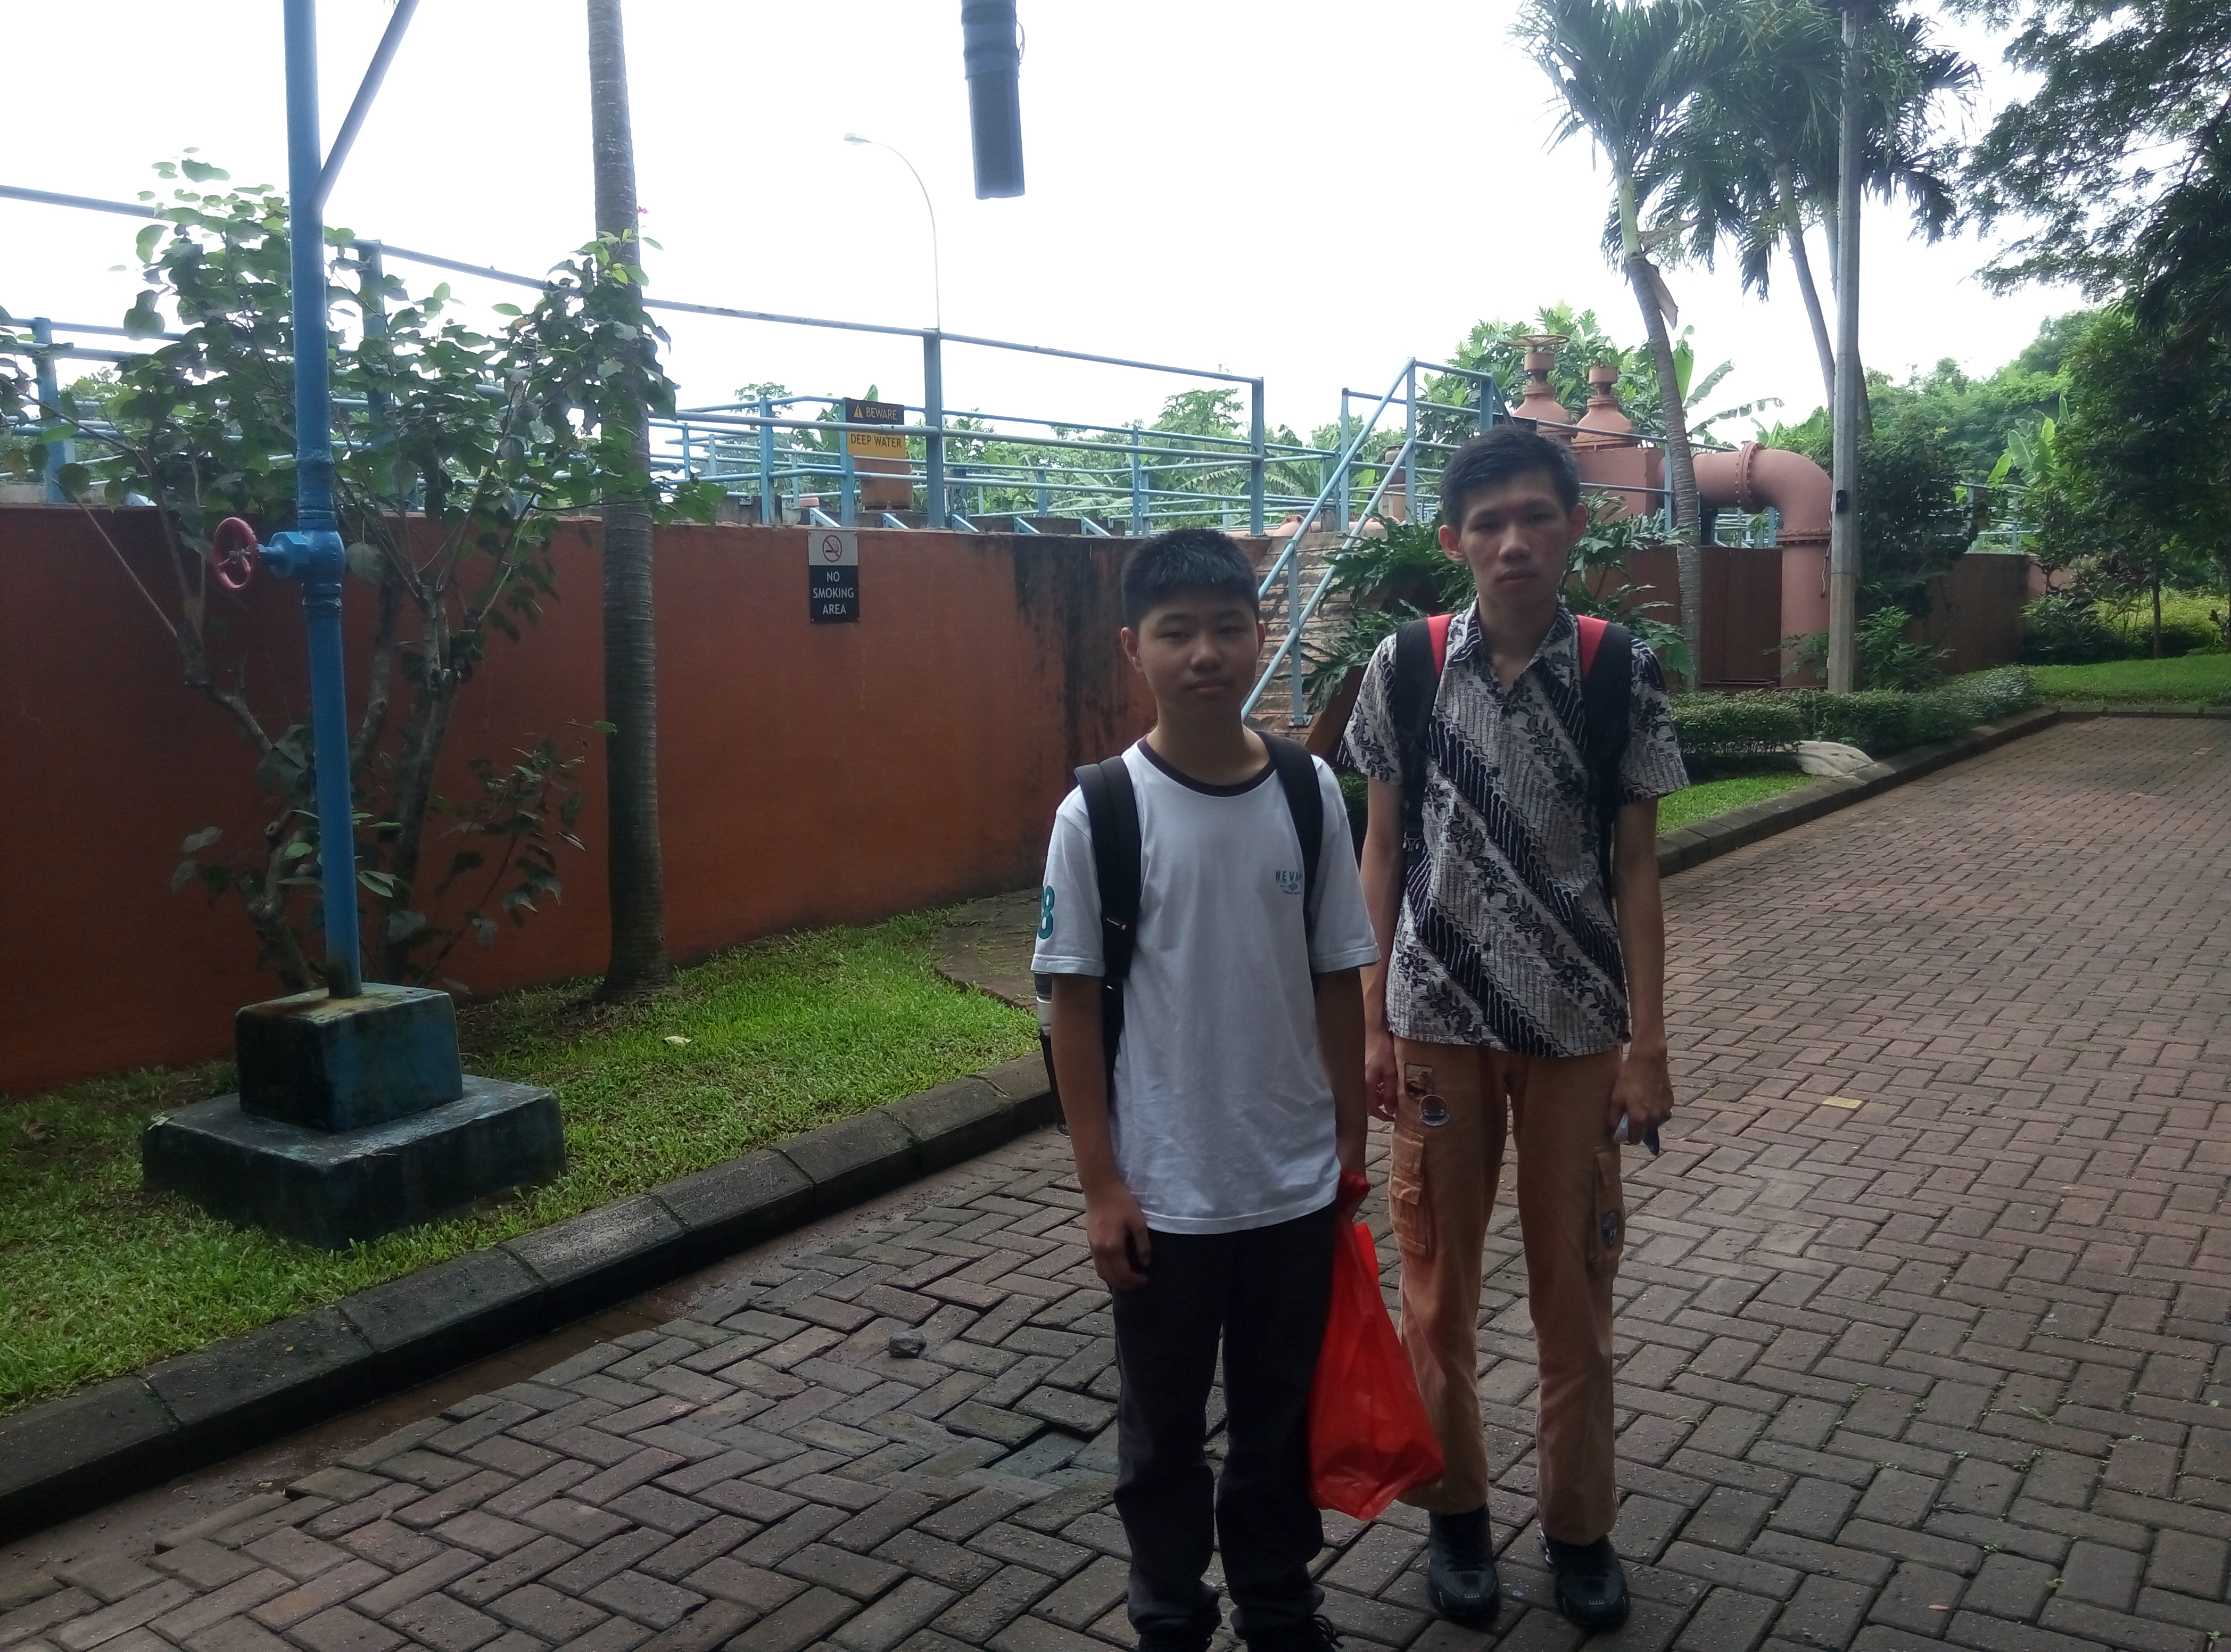
\includegraphics[width=\textwidth]{gfx/a1}
	\end{figure}
    \begin{figure}[!ht]
	  \centering
		  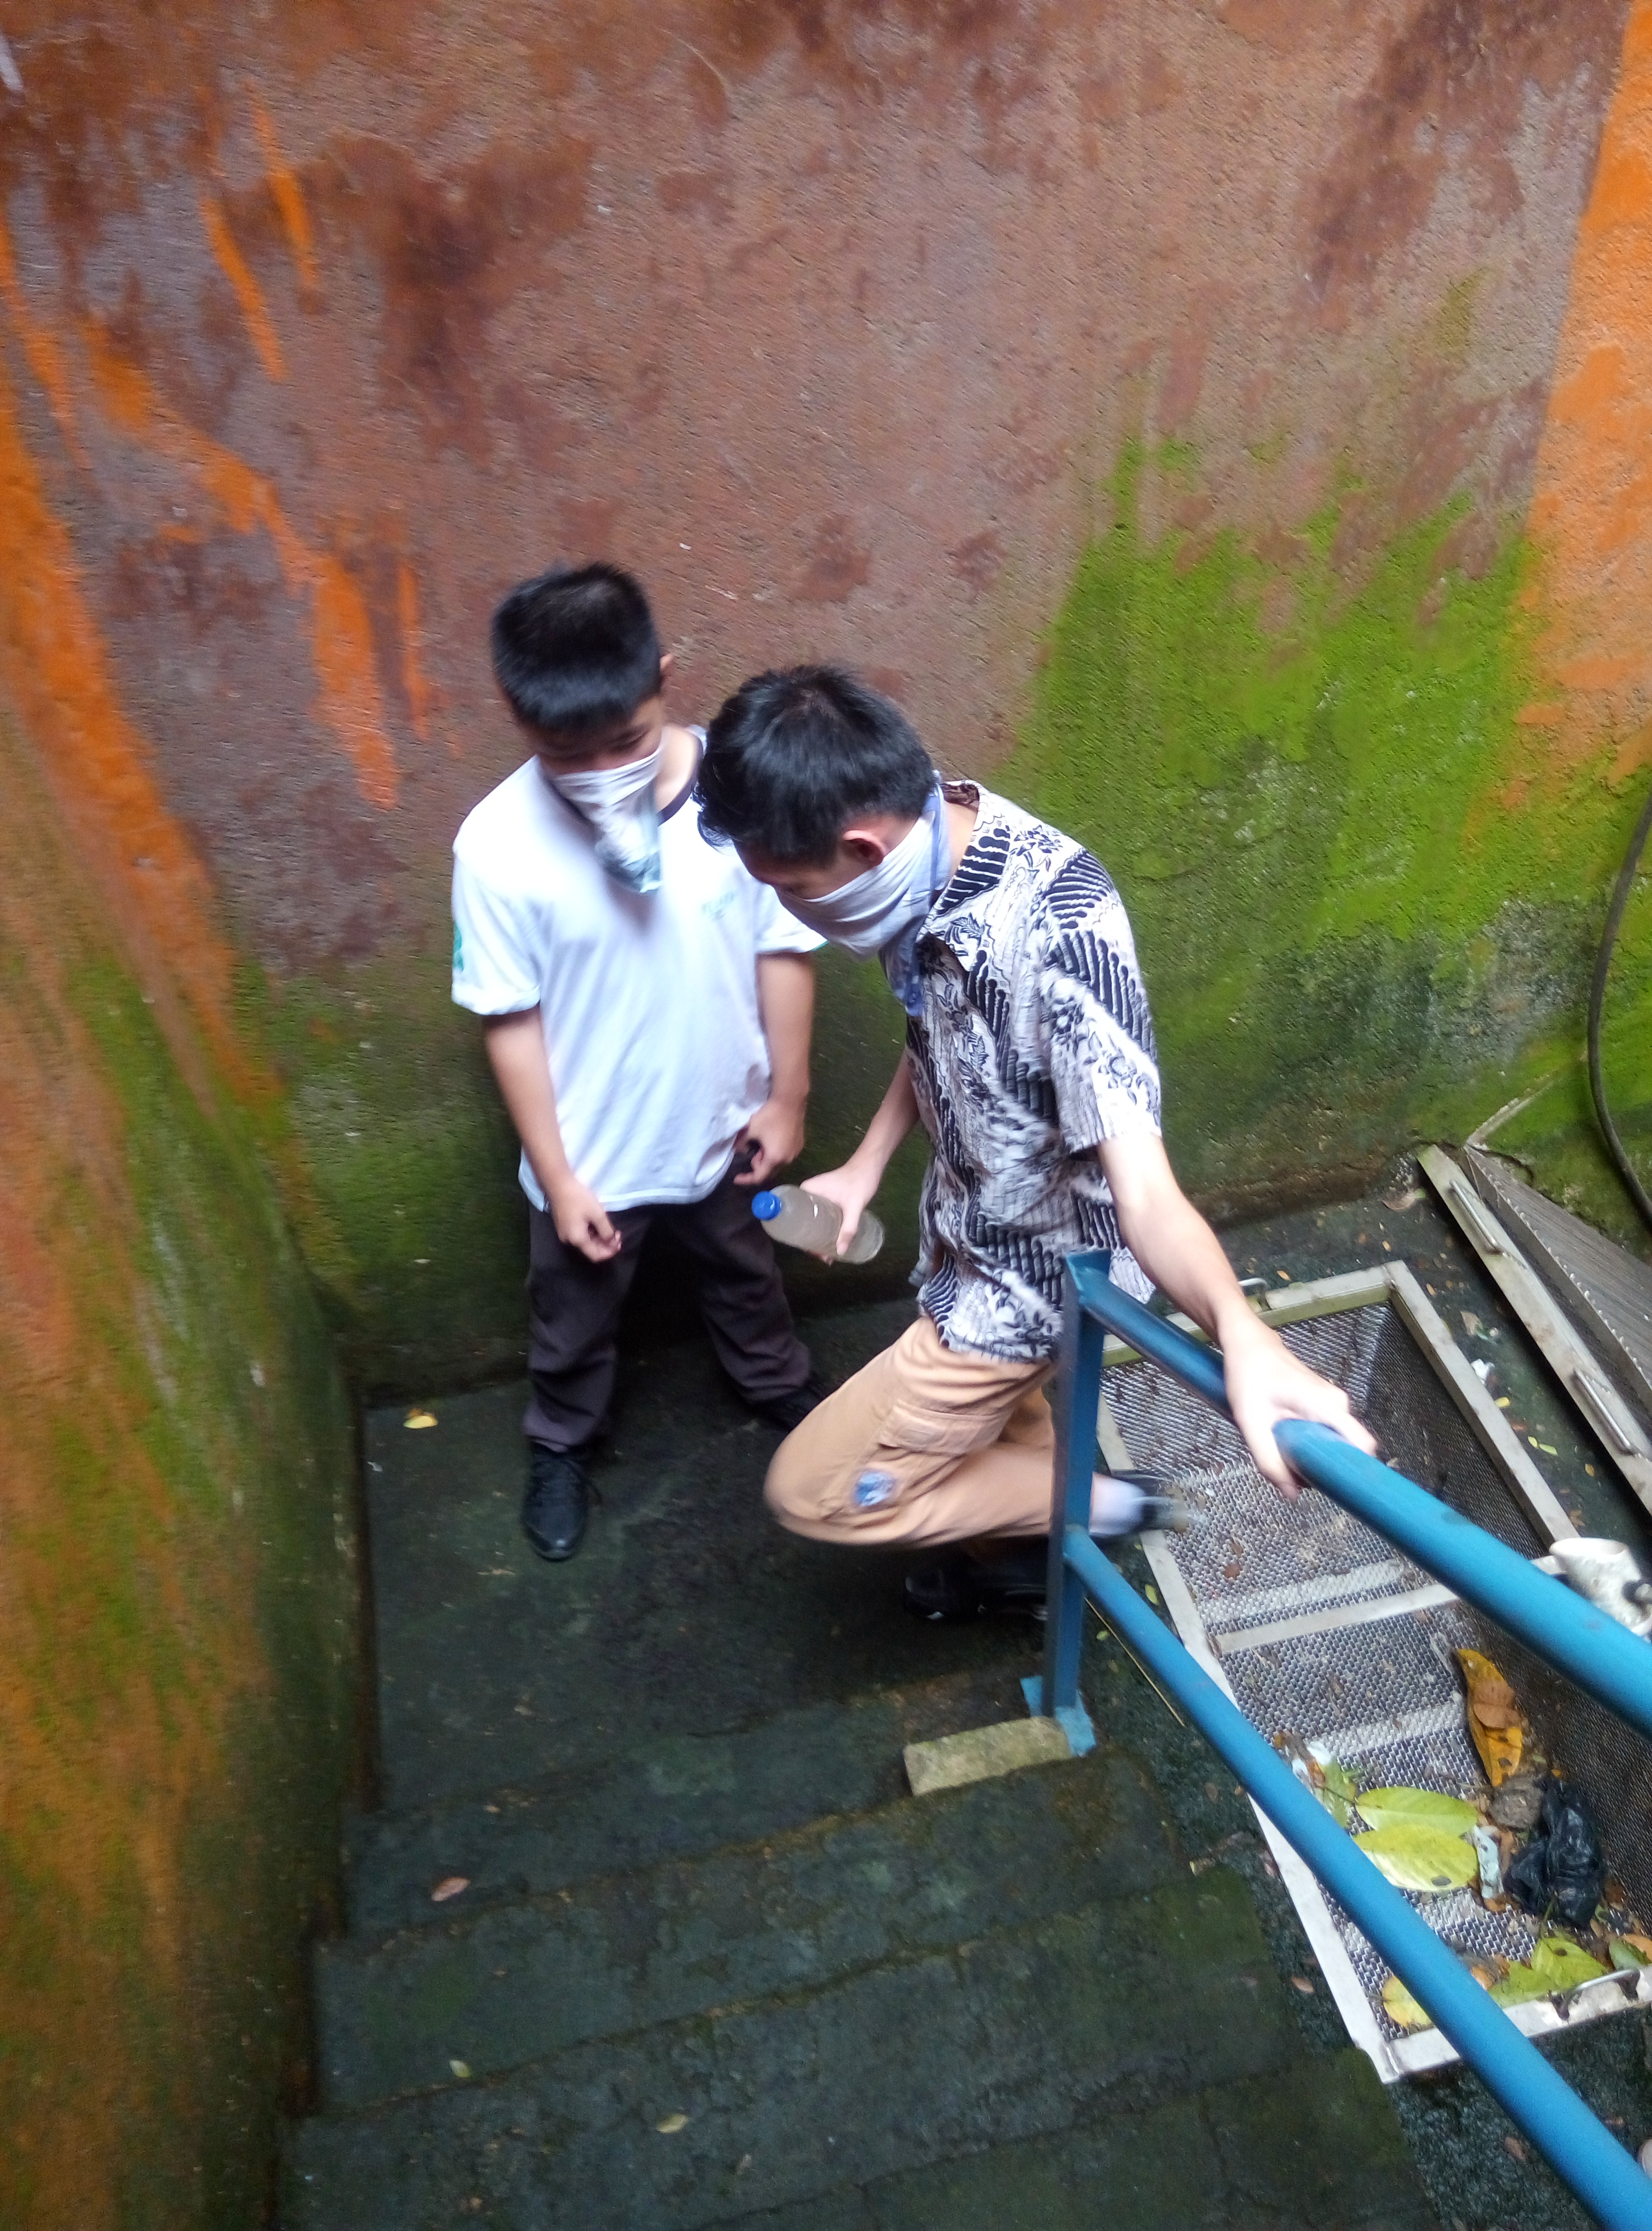
\includegraphics[width=\textwidth]{gfx/a2}
	\end{figure}	
    \begin{figure}[!ht]
	  \centering
		  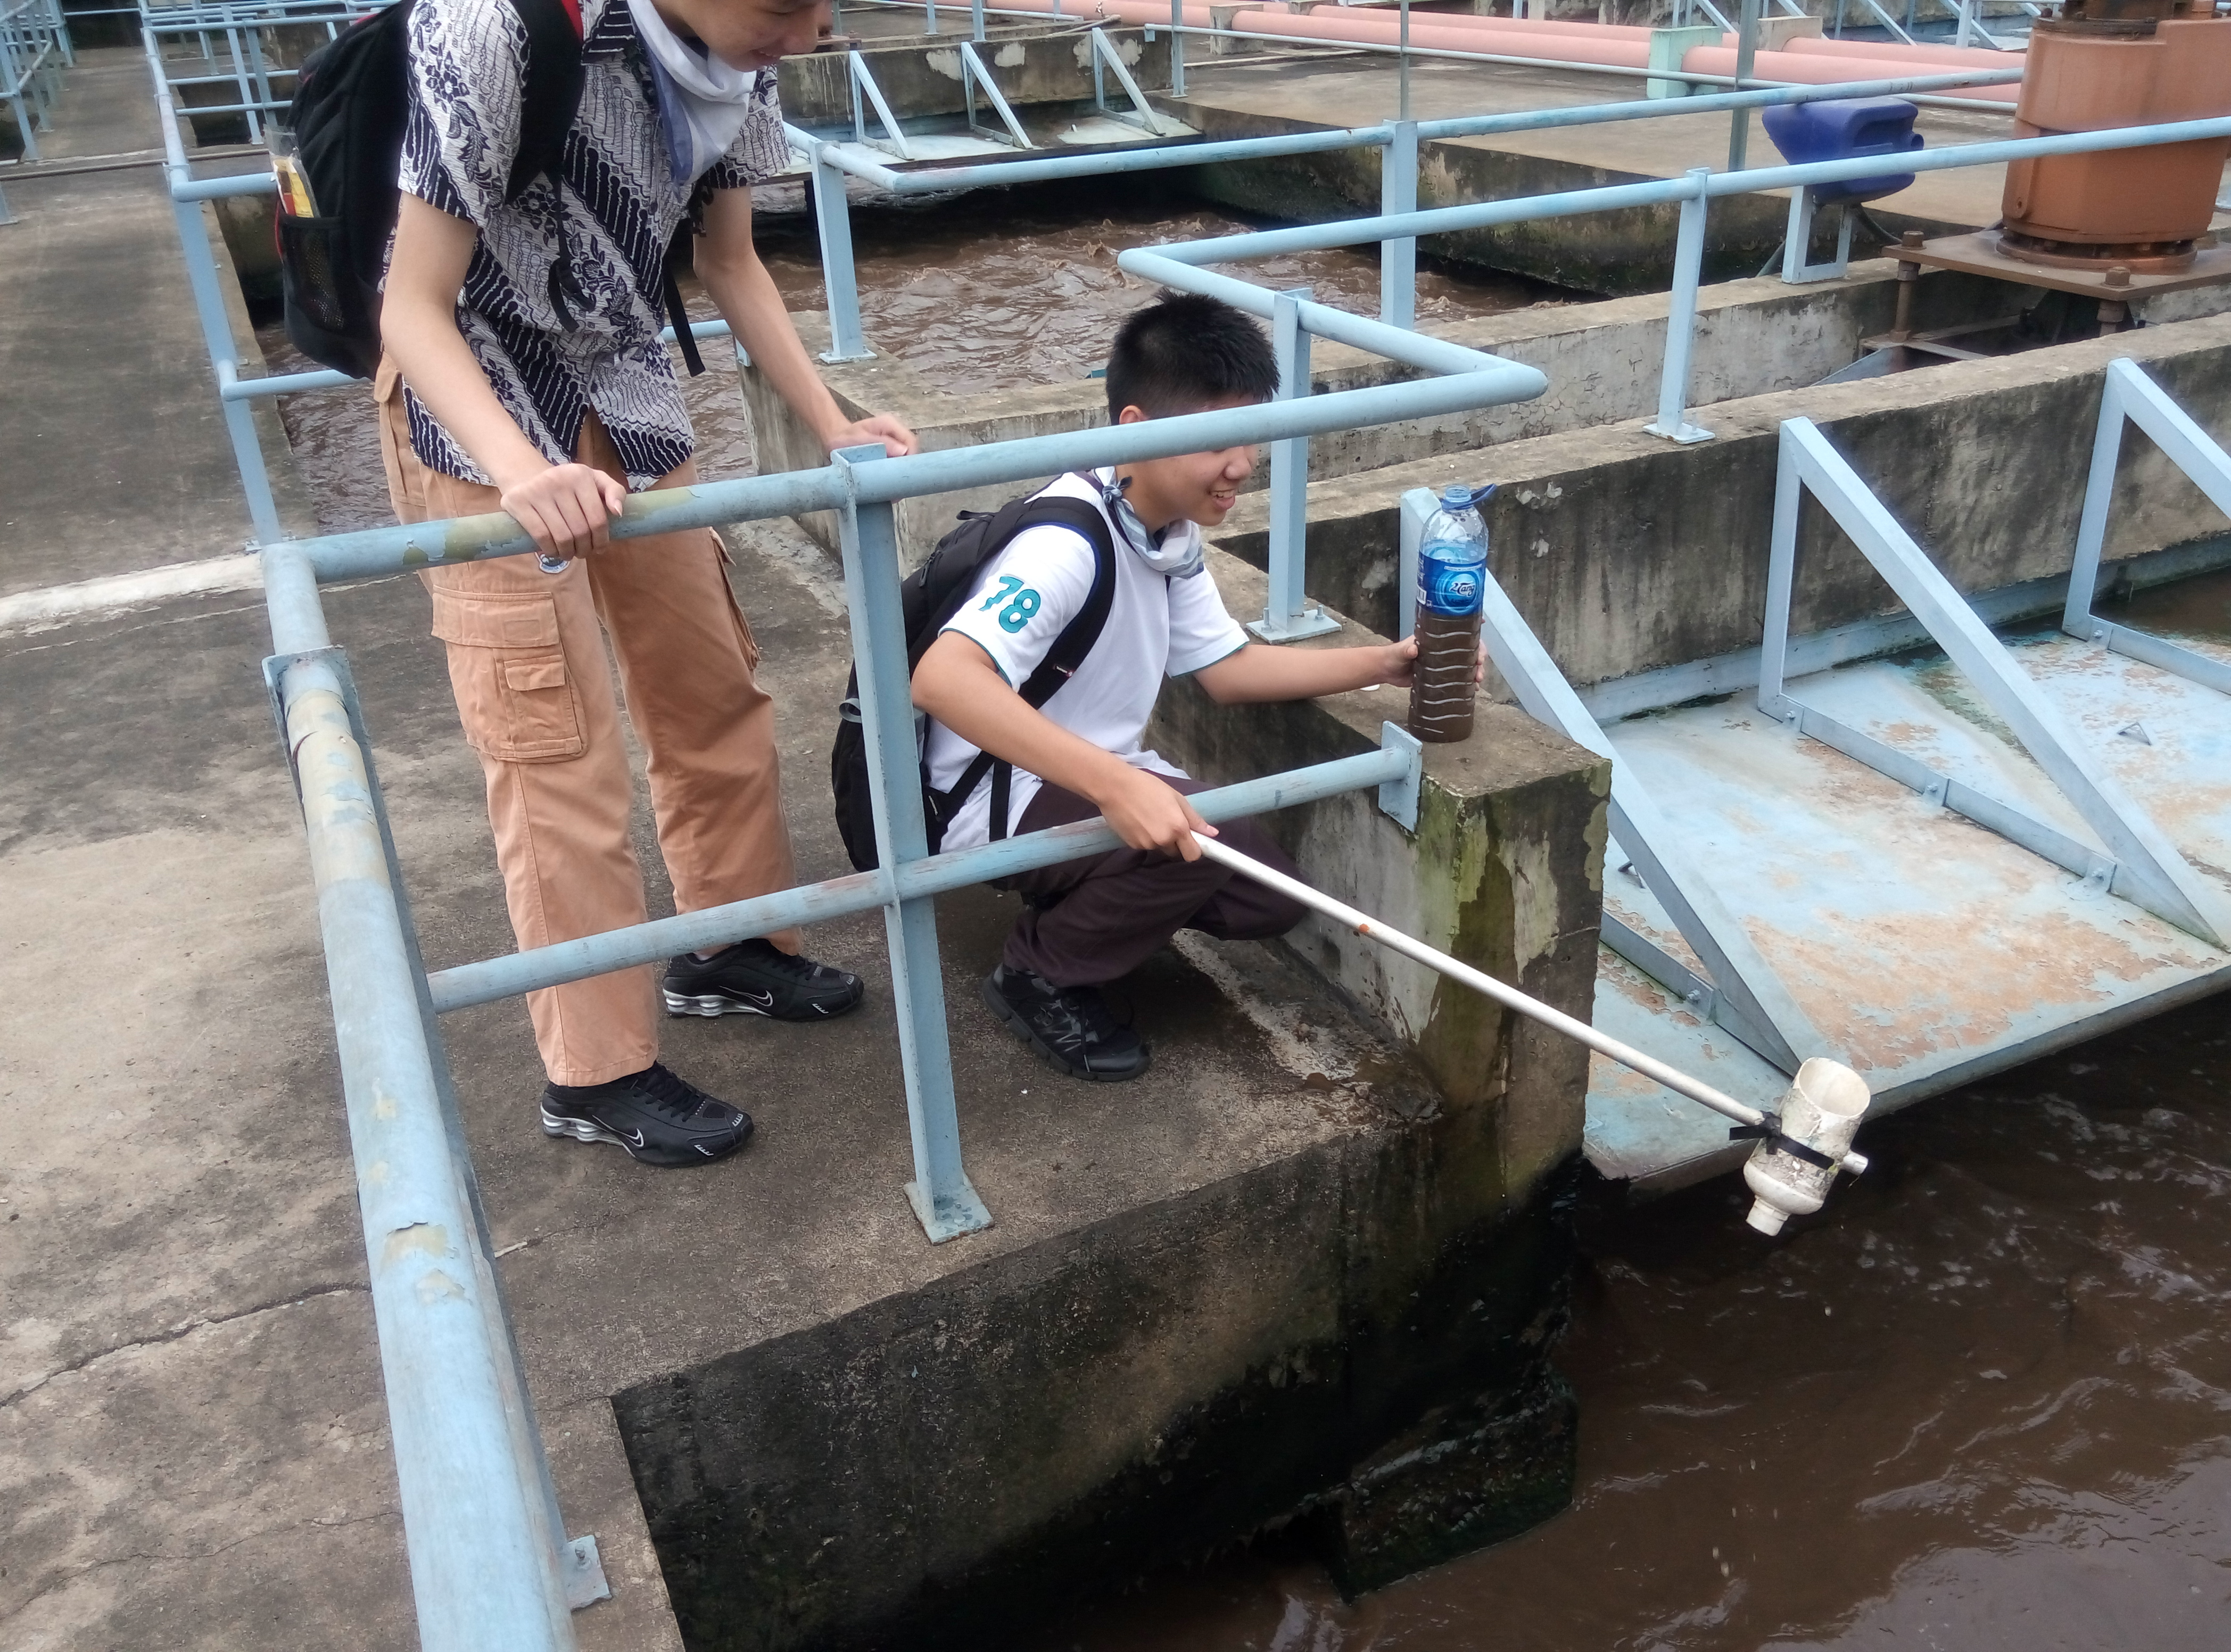
\includegraphics[width=\textwidth]{gfx/a3}
	\end{figure}    \begin{figure}[!ht]
	  \centering
		  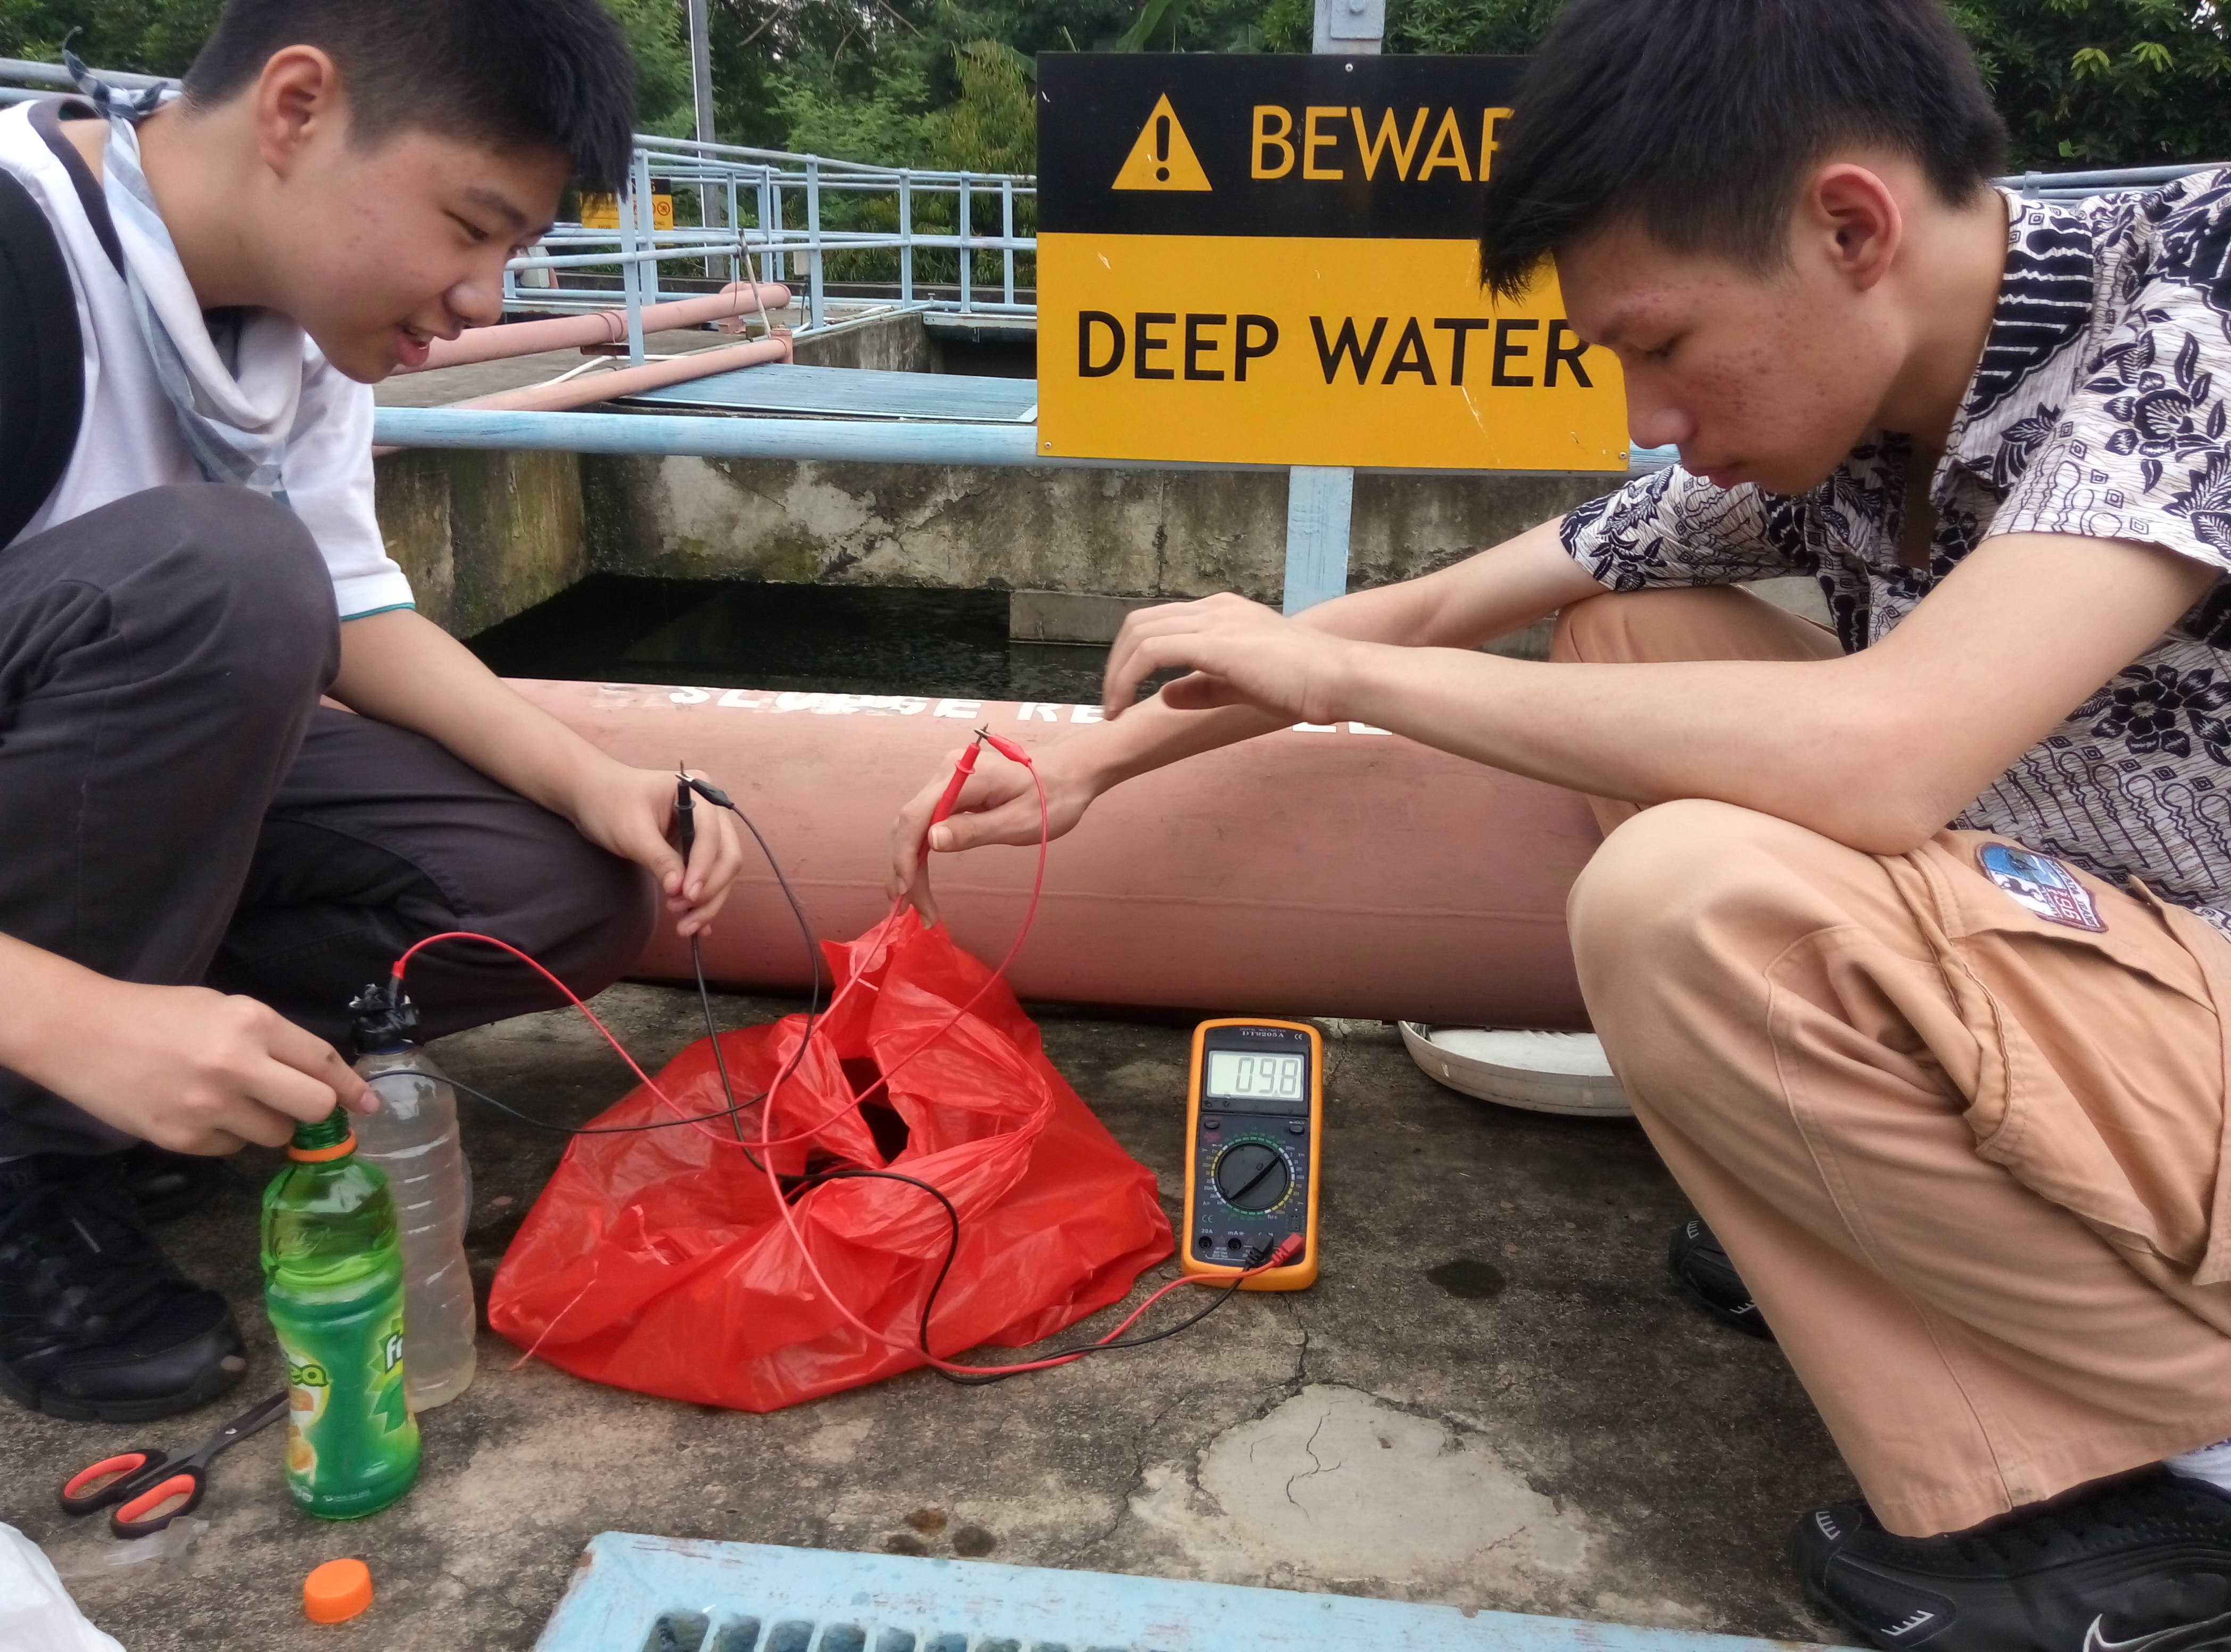
\includegraphics[width=\textwidth]{gfx/a4}
	\end{figure}	
    % Bibliography
    \nocite{*}
    \addtocontents{toc}{\protect\vspace{\beforebibskip}}
    \addcontentsline{toc}{section}{\refname}    
    \bibliographystyle{babplain}
    \bibliography{Bibliography}
\end{document}